


\section{DESIGN}

ThunderLoc adopts the client-server system architecture to allow transmission of data from the mobile devices to a server station or cloud platform.
When a thunder occurs, the smartphones will be triggered to transmit their positions, directions and binary measurement data to the server. 
The server will subsequently process the received data to implement thunder localization. 
In this section, we firstly introduce the design of client application, then two localization methods in the server end are introduced in the next two subsections.
  \vspace{-3mm}
\subsection{Data collection on client end}
  \vspace{-0mm}
  
Screen shots of the application and visualizations
used by the participants of the thunder can be seen in
Fig. \ref{Screen}. Fig. \ref{Dual}. shows the two channel sound signals from dual-microphone in a mobile phone.
It is easy to see that the thunder firstly reaches the microphone that corresponding to the top channel.

  \begin{figure}[hptb]
            \setlength{\abovecaptionskip}{0pt}
            \centering
            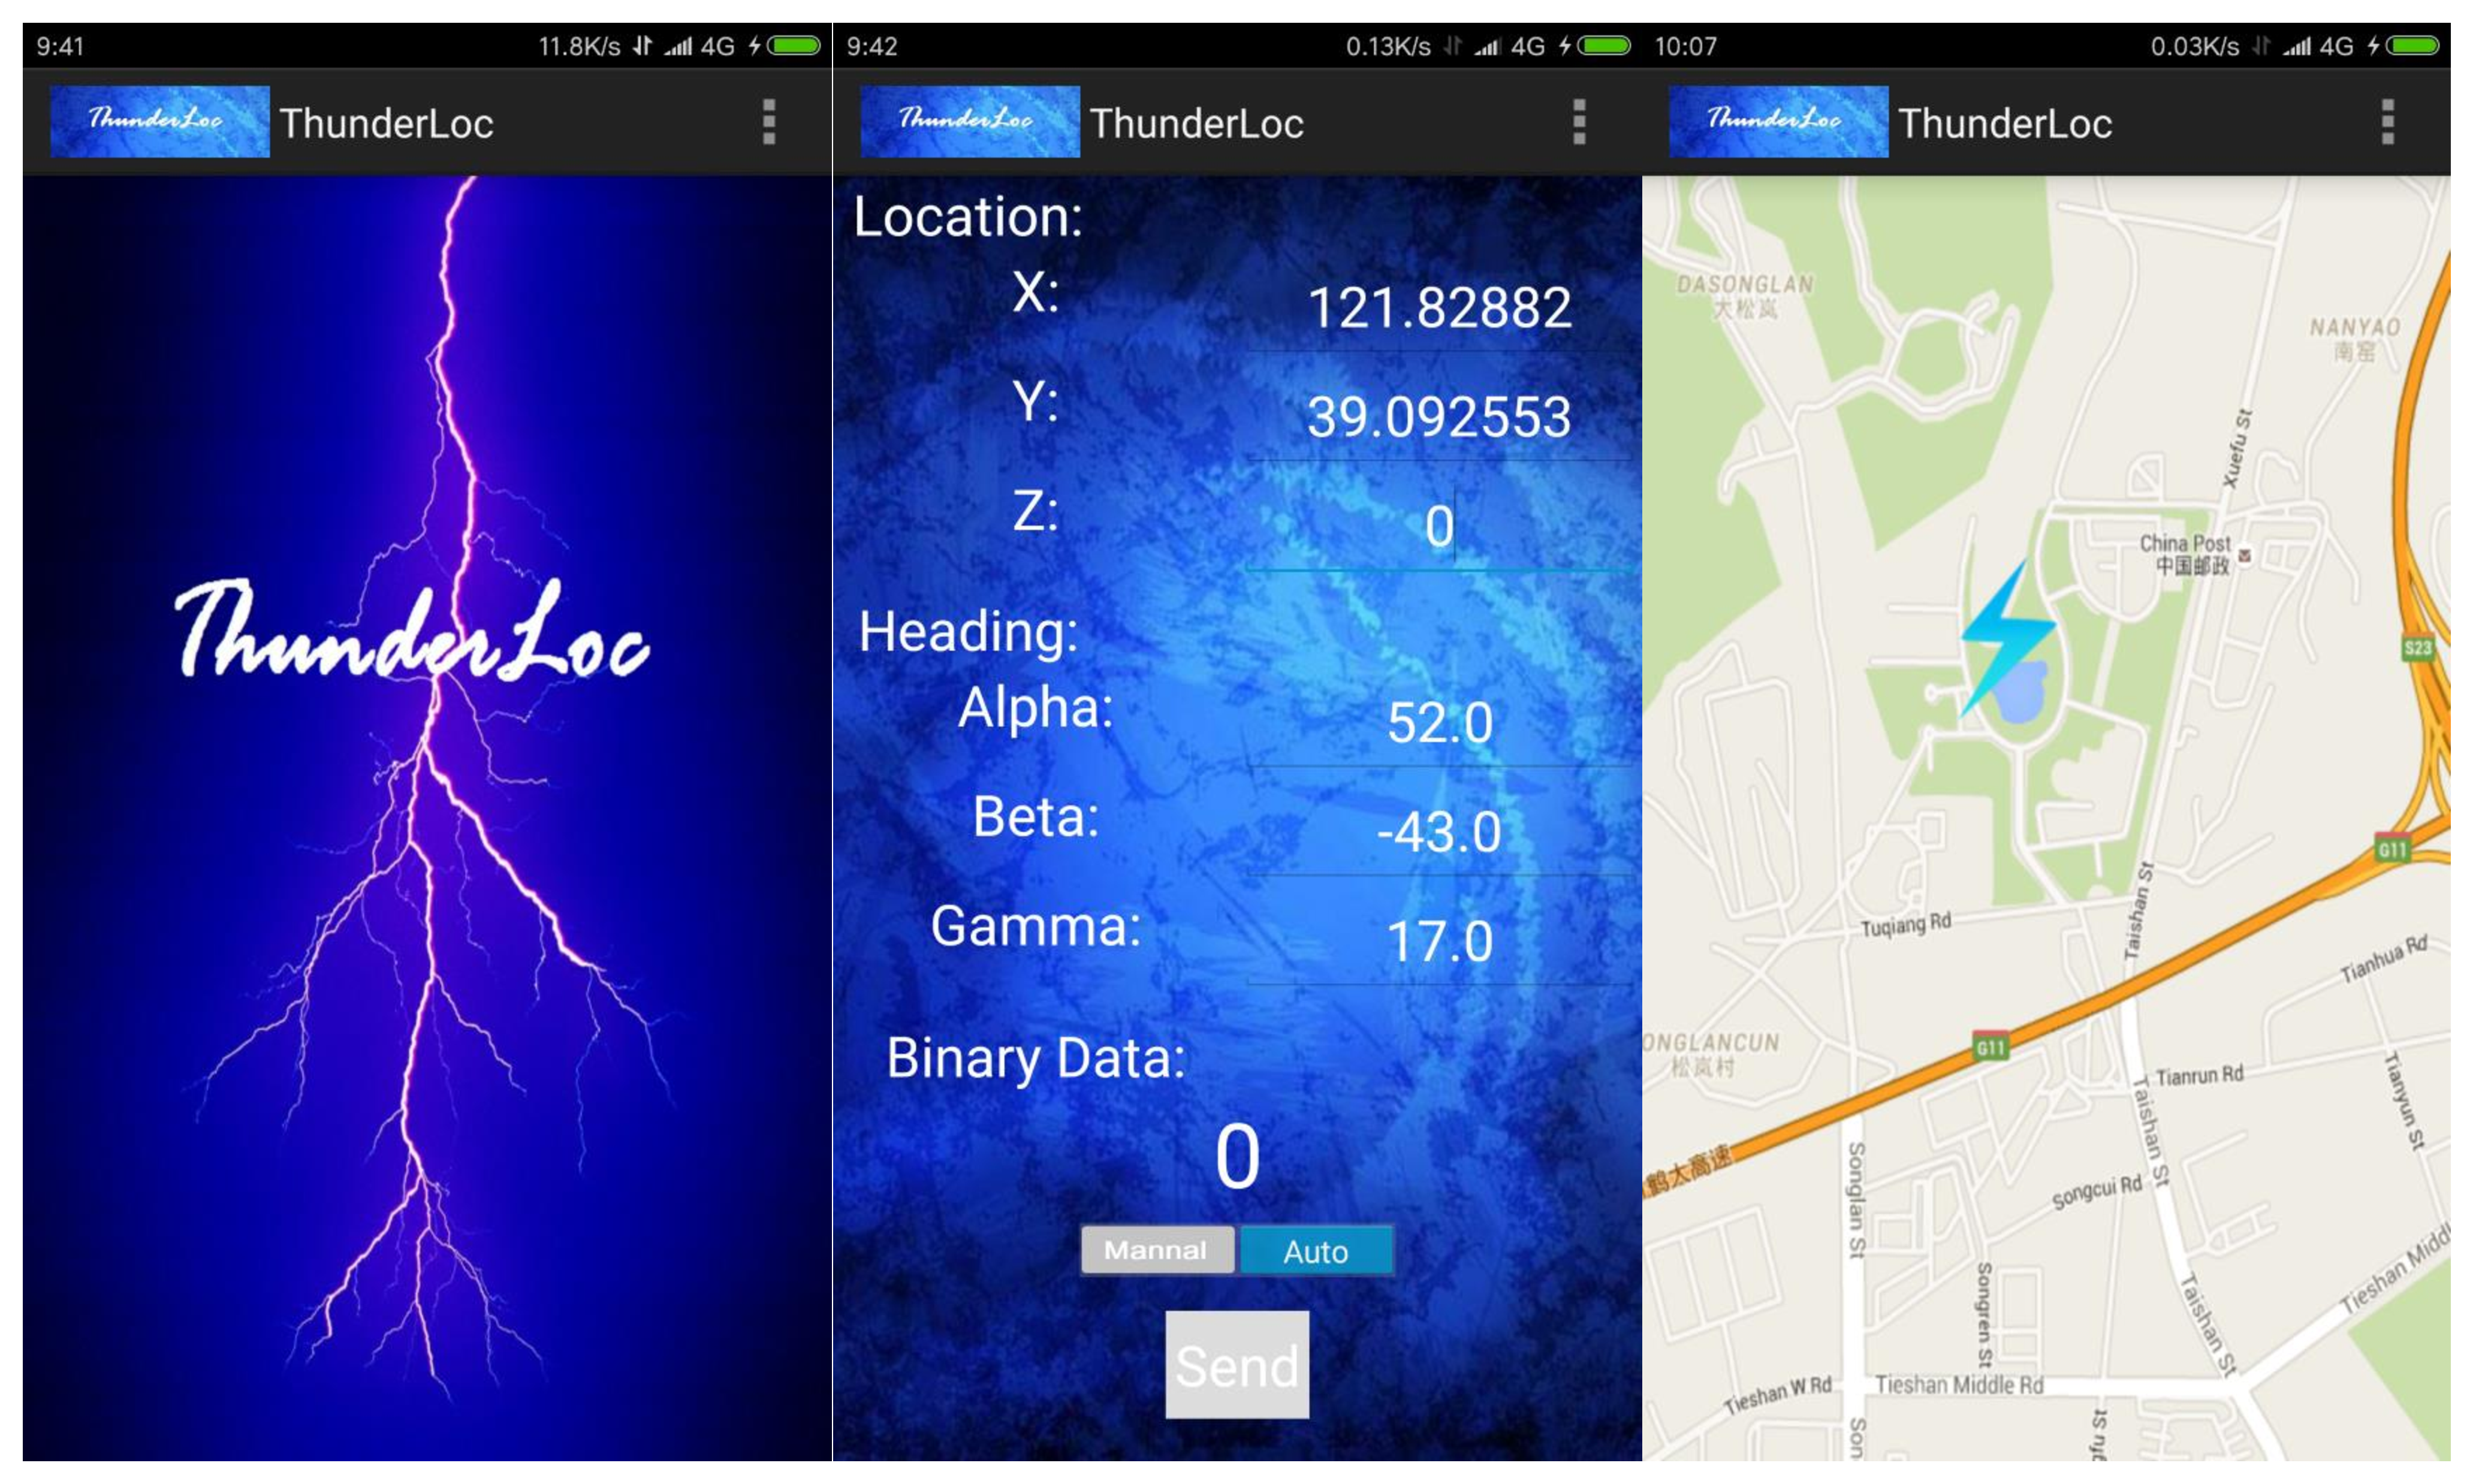
\includegraphics[scale=1.4,height=4.0cm]{fig/ThunderLoc.pdf}
			 \vspace{4mm}
            \caption{\label{Screen}Screen shots of ThunderLoc client application.}
            \vspace{-6mm}
  \end{figure}
  
  

  \begin{figure}[ht]
            \setlength{\abovecaptionskip}{0pt}
            \centering
            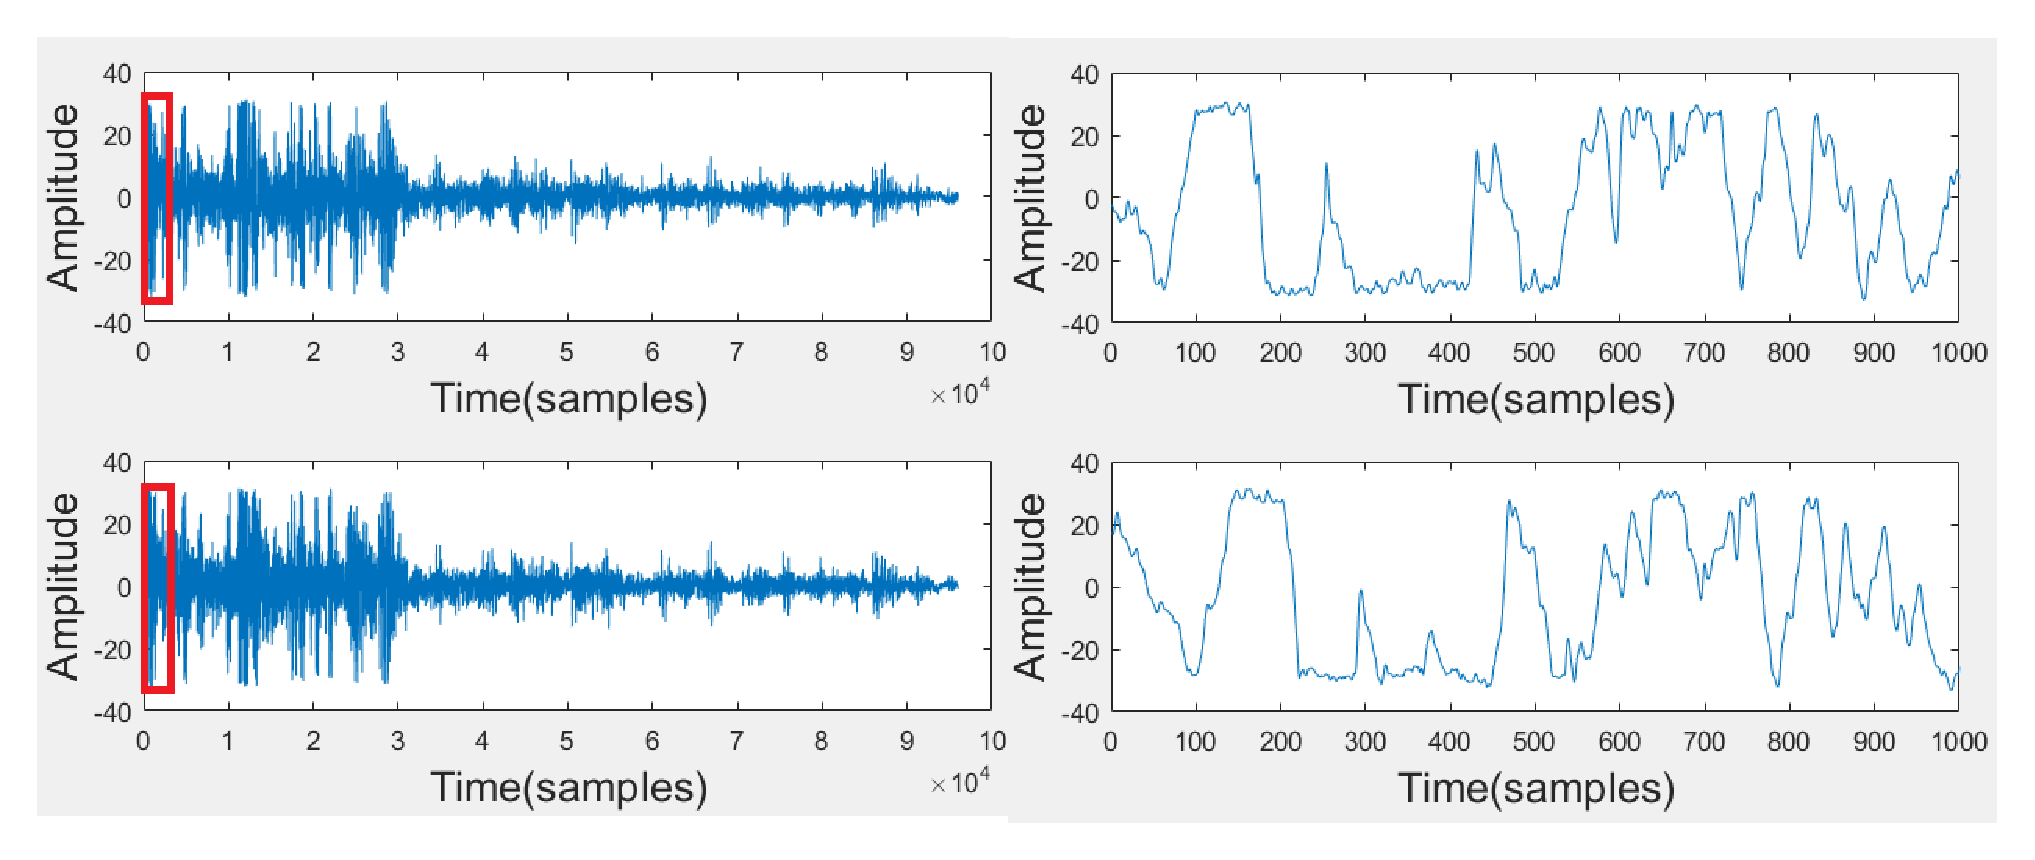
\includegraphics[width=9cm,height=4cm]{fig/dualmic.pdf}
     \vspace{2mm}
            \caption{Dual-microphone acoustic signals.}
            \label{Dual}
            \vspace{-2mm}
  \end{figure}



  \begin{figure}[ht]
            \setlength{\abovecaptionskip}{0pt}
            \centering
            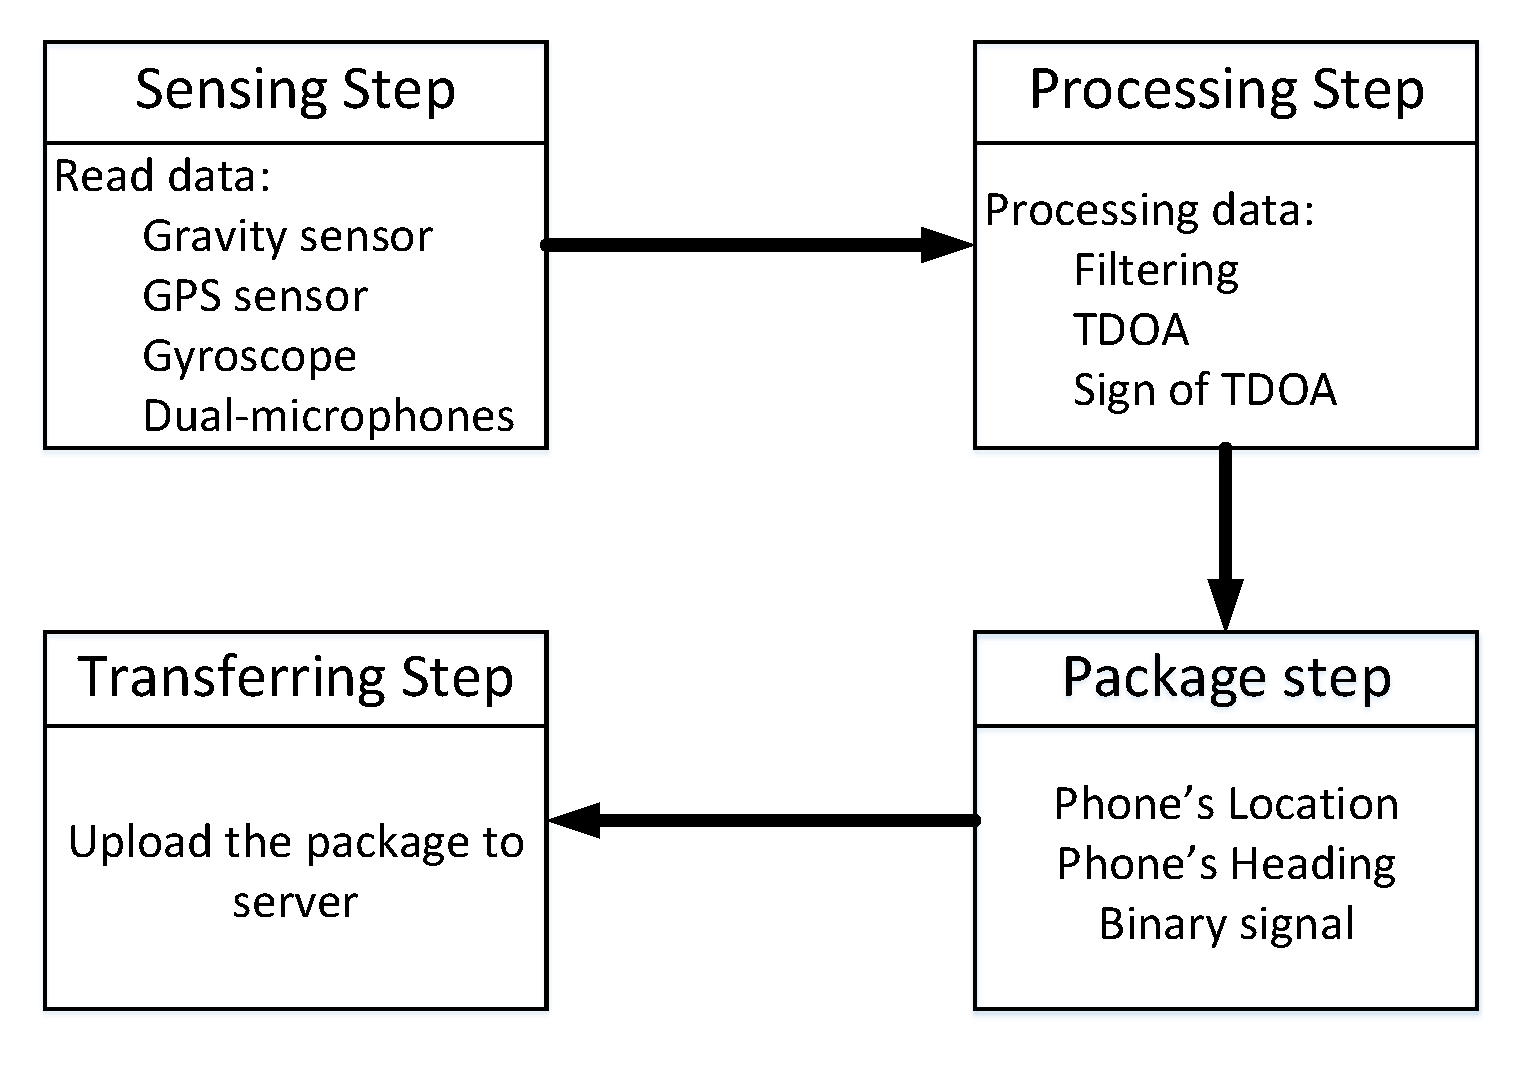
\includegraphics[scale=2,width=6.0cm]{fig/client.pdf}
     \vspace{2mm}
            \caption{The diagram of signal processing of acoustic signals.}
            \label{Diagram}
            \vspace{-4mm}
  \end{figure}



Fig. \ref{Diagram} depicts the flow of the ThunderLoc client application. 
ThunderLoc client application has two main independent threads: sensing thread and
communication thread. The sensing thread handles the interaction
with the main application and the on-board sensors, the communication thread
handles local storage, transmission of recorded sensor events and requeues of events in the case of poor network connection. 
Considering the energy problem, it is not an energy-effective solution for the mobile devices to continuously send
data to the servers. To deal with this issue, a three-state model is
used for ThunderLoc client application: Idle Mode, Listening Mode and Communication Mode. 
Fig. \ref{Mode} depicts the different modes of sensing of the client end.
While continuously recording and sensing for probable thunder events locally on the mobile phones, this model permits minimal transmission of data to the server. 
 

  \begin{figure}[ht]
            \setlength{\abovecaptionskip}{0pt}
            \centering
            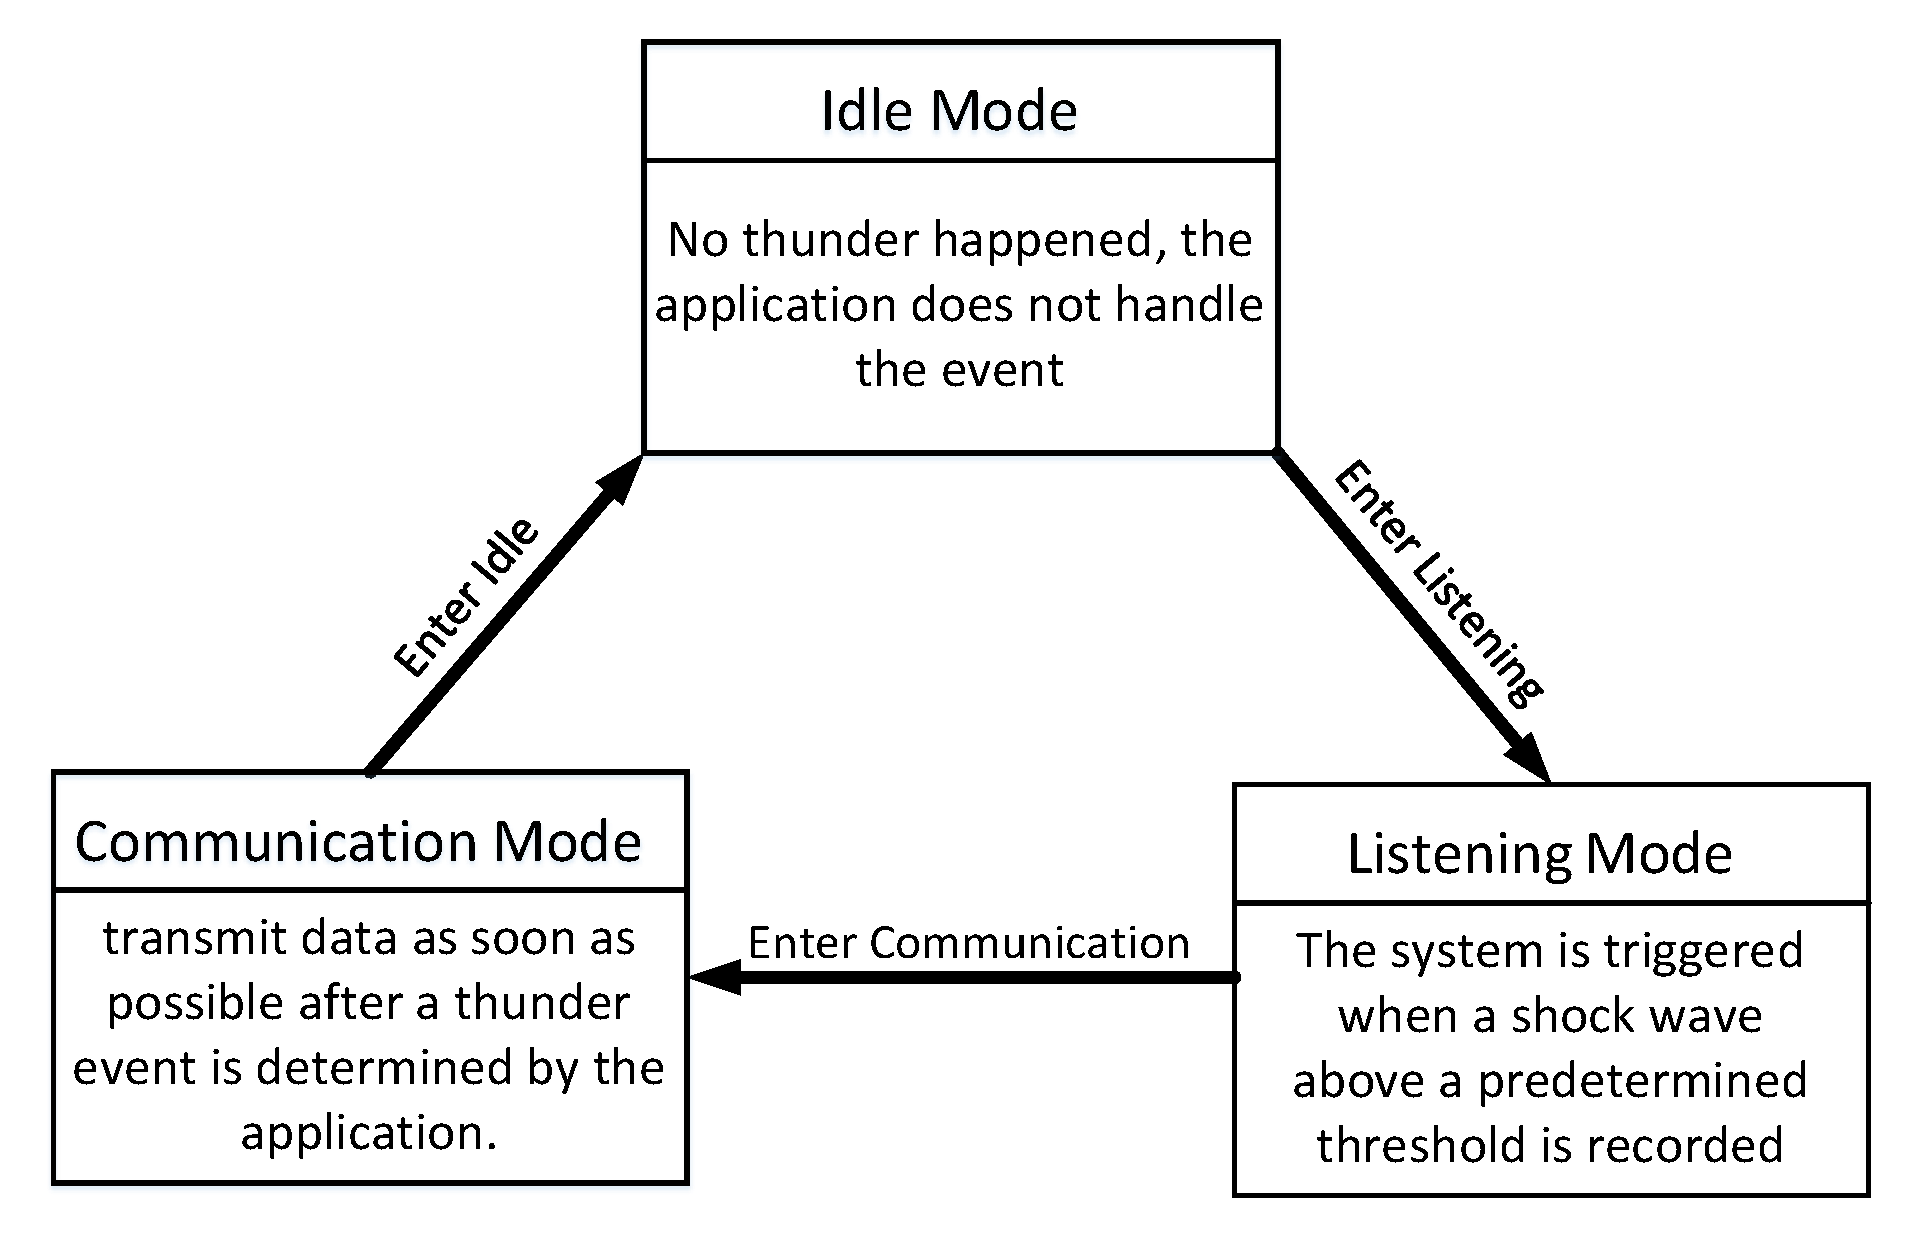
\includegraphics[scale=1.4,height=4.0cm]{fig/modechange.pdf}
     \vspace{4mm}
            \caption{Modes of sensing of the client end}
            \label{Mode}
            \vspace{-4mm}
  \end{figure}


1) Idle Mode:
In order to determine the orientation of a mobile phone, the mobile device must be stationary for a period of time while recording the sensor data. 
Device movement is characterized by a change in the readings of the accelerometer and gyroscope. 
If the cumulative movement is under the threshold, the device will be verified as still, then jumps into the listening mode.

2) Listening Mode:
Thunder is the acoustic shock wave resulted from a sudden and intense heating of the air in the lightning channel. 
%The application is able to capture the shock wave by always keeping recoding a
%segment of the signal in a circular memory buffer before the threshold triggering of the system. 
The system is triggered when a shock wave above a predetermined threshold is recorded. 
Specially, the trigger is fired when an average energy is rising 4 times experienced by any of
the dual microphones. 

3) Communication Mode: To reduce the total latency of the ThunderLoc system, it is necessary to transmit data as soon as possible after
a thunder event occurs. 
The application records sensor readings about heading and location of the smartphone, then immediately transmits these data to the server along with the binary measurement data estimated from two channel acoustic signals of dual microphones.
In case the communication service is not available during the thunder event, a copy of these recordings is stored locally, then placed into a queue to be sent once communication is available again.

Besides the implicit way to collect data, 
ThunderLoc also allows user to explicitly input location, 
direction and binary measurement data by the way of `humans as sensor'~\cite{wang2014using}. %~\cite{wang2014using,resch2013people}

%~\cite{wang2014using,resch2013people}.



 
  \vspace{-1mm}
\subsection{Basic localization on server side}
  \vspace{-0mm}
  
    \begin{figure}[ht]
            \setlength{\abovecaptionskip}{0pt}
            \centering
            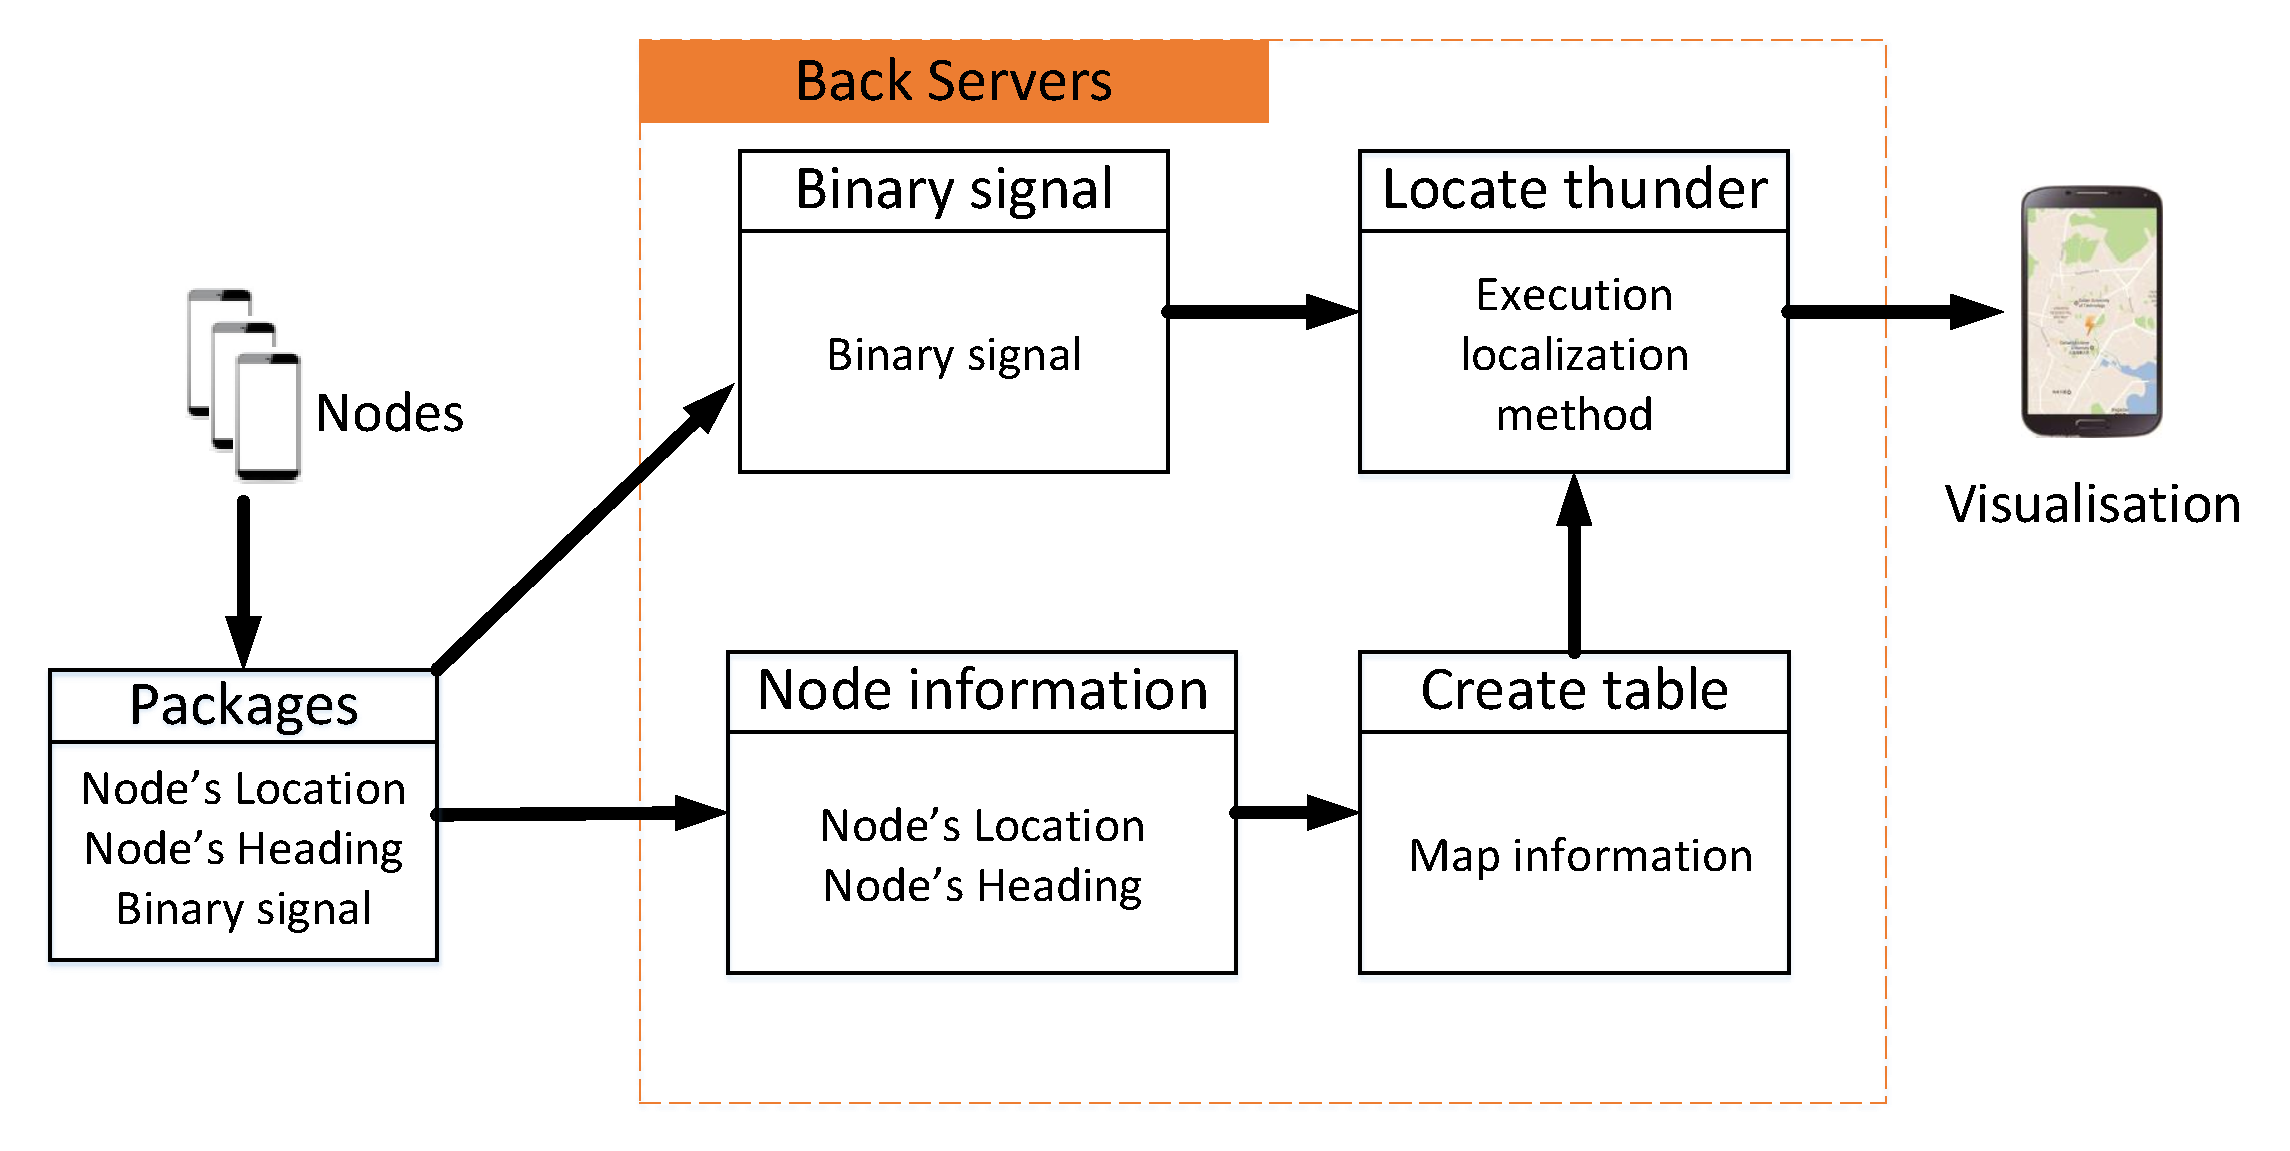
\includegraphics[scale=1.4,height=4.0cm]{fig/server.pdf}
     \vspace{4mm}
            \caption{The diagram at cloud platform.}
            \label{Server}
            \vspace{-4mm}
  \end{figure}

  
In this section, the position and orientation of a smartphone are assumed to be known, which can be estimated by its GPS(or Wi-Fi based indoor localization) and motion sensors, respectively.
Fig. \ref{Server} depicts the flow of the ThunderLoc server application. In the cloud computing platform, the map of space division can be built with the position and orientation information of all smartphone nodes.
Then, we can turn the acoustic source localization into the searching problem in the Hamming space. 

Firstly, we introduce the basic localization method. Let us consider the 4G network with $N$ dual-microphone smartphones randomly deployed in 2D area. 
The top-level idea for basic ThunderLoc is to split the whole localization area into some subregions identified by respective binary sequences.
Given $N$ smartphone nodes in the localization space, the whole number of combinations of binary sequences is $2^N$ in theory.
However, in the practical system, given $N$ smartphone nodes in the localization space,
the possible number of combinations of binary sequences is only $(N^2+N+2)/2$.
The lower dimensionality of the sequence table enables the correction of errors in the measured sequence.
This is one of the reasons that our proposed algorithm performs well in adverse conditions.
Localization system can achieve higher localization performance as the number of smartphones increases, such extensibility is an unique advantage compared with dedicated microphone array hardware.



\textbf{Binary sensor model}:
 We propose a binary sensor model, where the TDOA of dual-channel acoustic signals is converted reliably to one bit of information: the thunder is on the left or right of the perpendicular bisector of dual-microphones. 
We use the sign of TDOA as 1 bit measurement information, which reveals the left/right information about the direction of the incoming Thunder.
Using 1-bit measurement information allows for inexpensive sensing as well as minimal communication load.
As shown in Fig. 2, for each dual-microphone smartphone node, 
TDOA is computed by traditional time delay estimation method (such as generalized cross correlation, GCC), % ~\cite{knapp1976generalized}
then we can get the binary sequence of the thunder.

  \begin{figure}[ht]
            \setlength{\abovecaptionskip}{0pt}
            \centering
            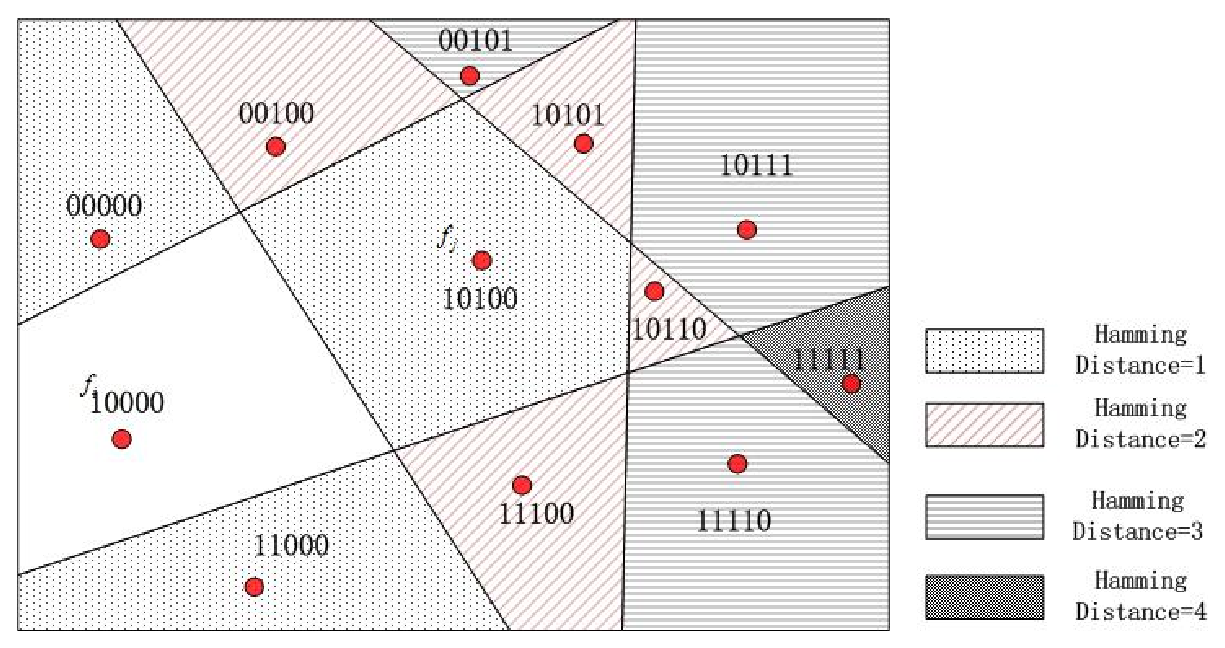
\includegraphics[scale=1.4,height=4.0cm]{image/Hamming_distance2.eps}
     \vspace{4mm}
            \caption{Hamming distance vs. geographic distance.}
            \label{Hamming}
            \vspace{-8mm}
  \end{figure}

\textbf{Hamming distance}:
For two faces $f_i$ and $f_j$ in Fig. \ref{Hamming}, now there are two types
of distance: (i) the geographical distance $GD({f_i},{f_j})$ between the center points of ${f_i}$ and ${f_j}$, and (ii) the Hamming distance
$HD({f_i},{f_j})$. Hamming distance measures the number of dimensions where two vectors have different values. 

  
  
\begin{figure}[hptb]
 \setlength{\abovecaptionskip}{0pt}
	\begin{minipage}[t]{0.45\linewidth}
		\centering
		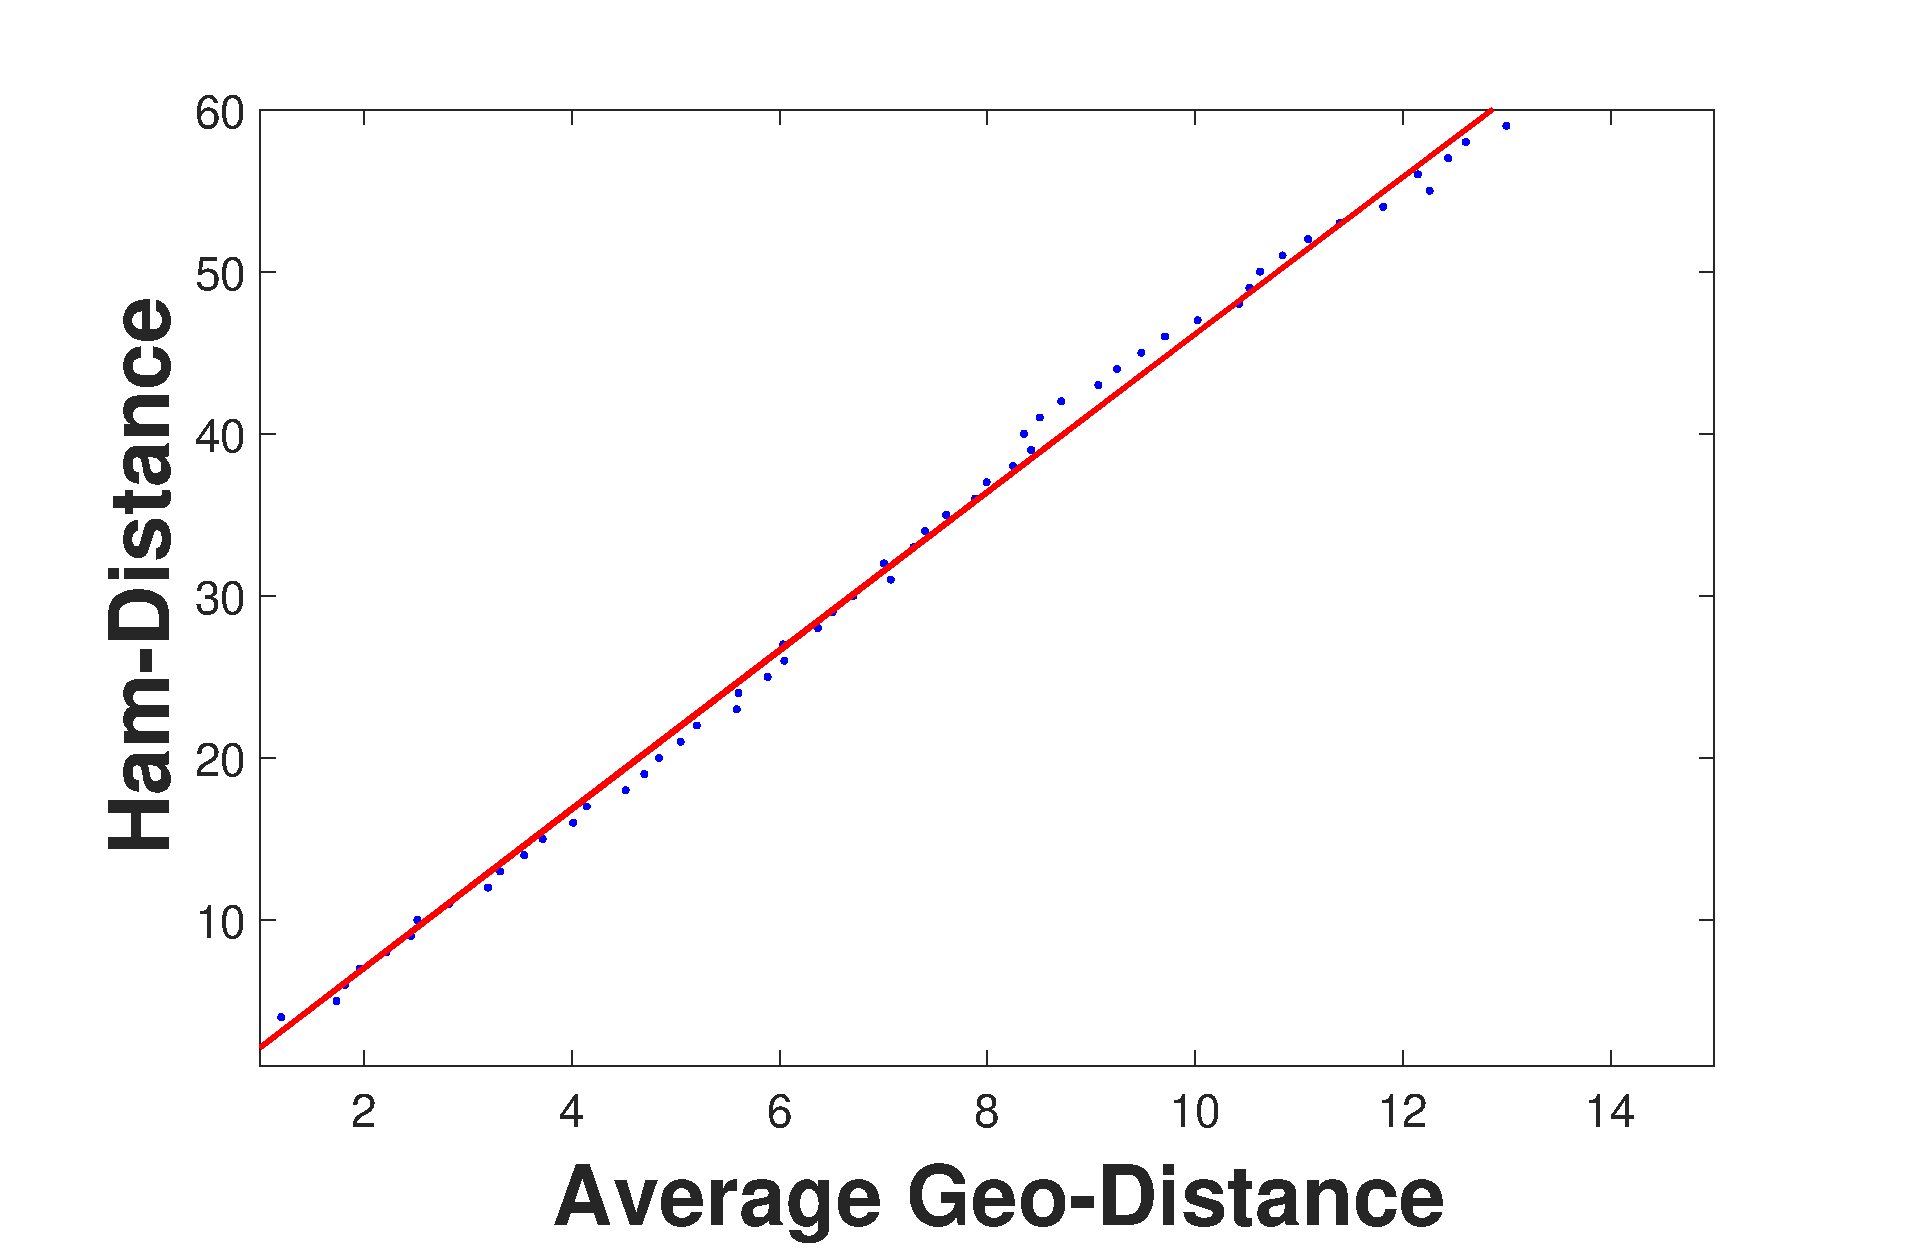
\includegraphics[height=2.85cm]{fig/Hamming1.eps}
		 \vspace{2mm}
	%	\caption{Hamming distance vs. Average geographic distance.}
	\vspace{-2mm}
	\end{minipage}%
		\hspace{1mm}
	\begin{minipage}[t]{0.45\linewidth}
		\centering
		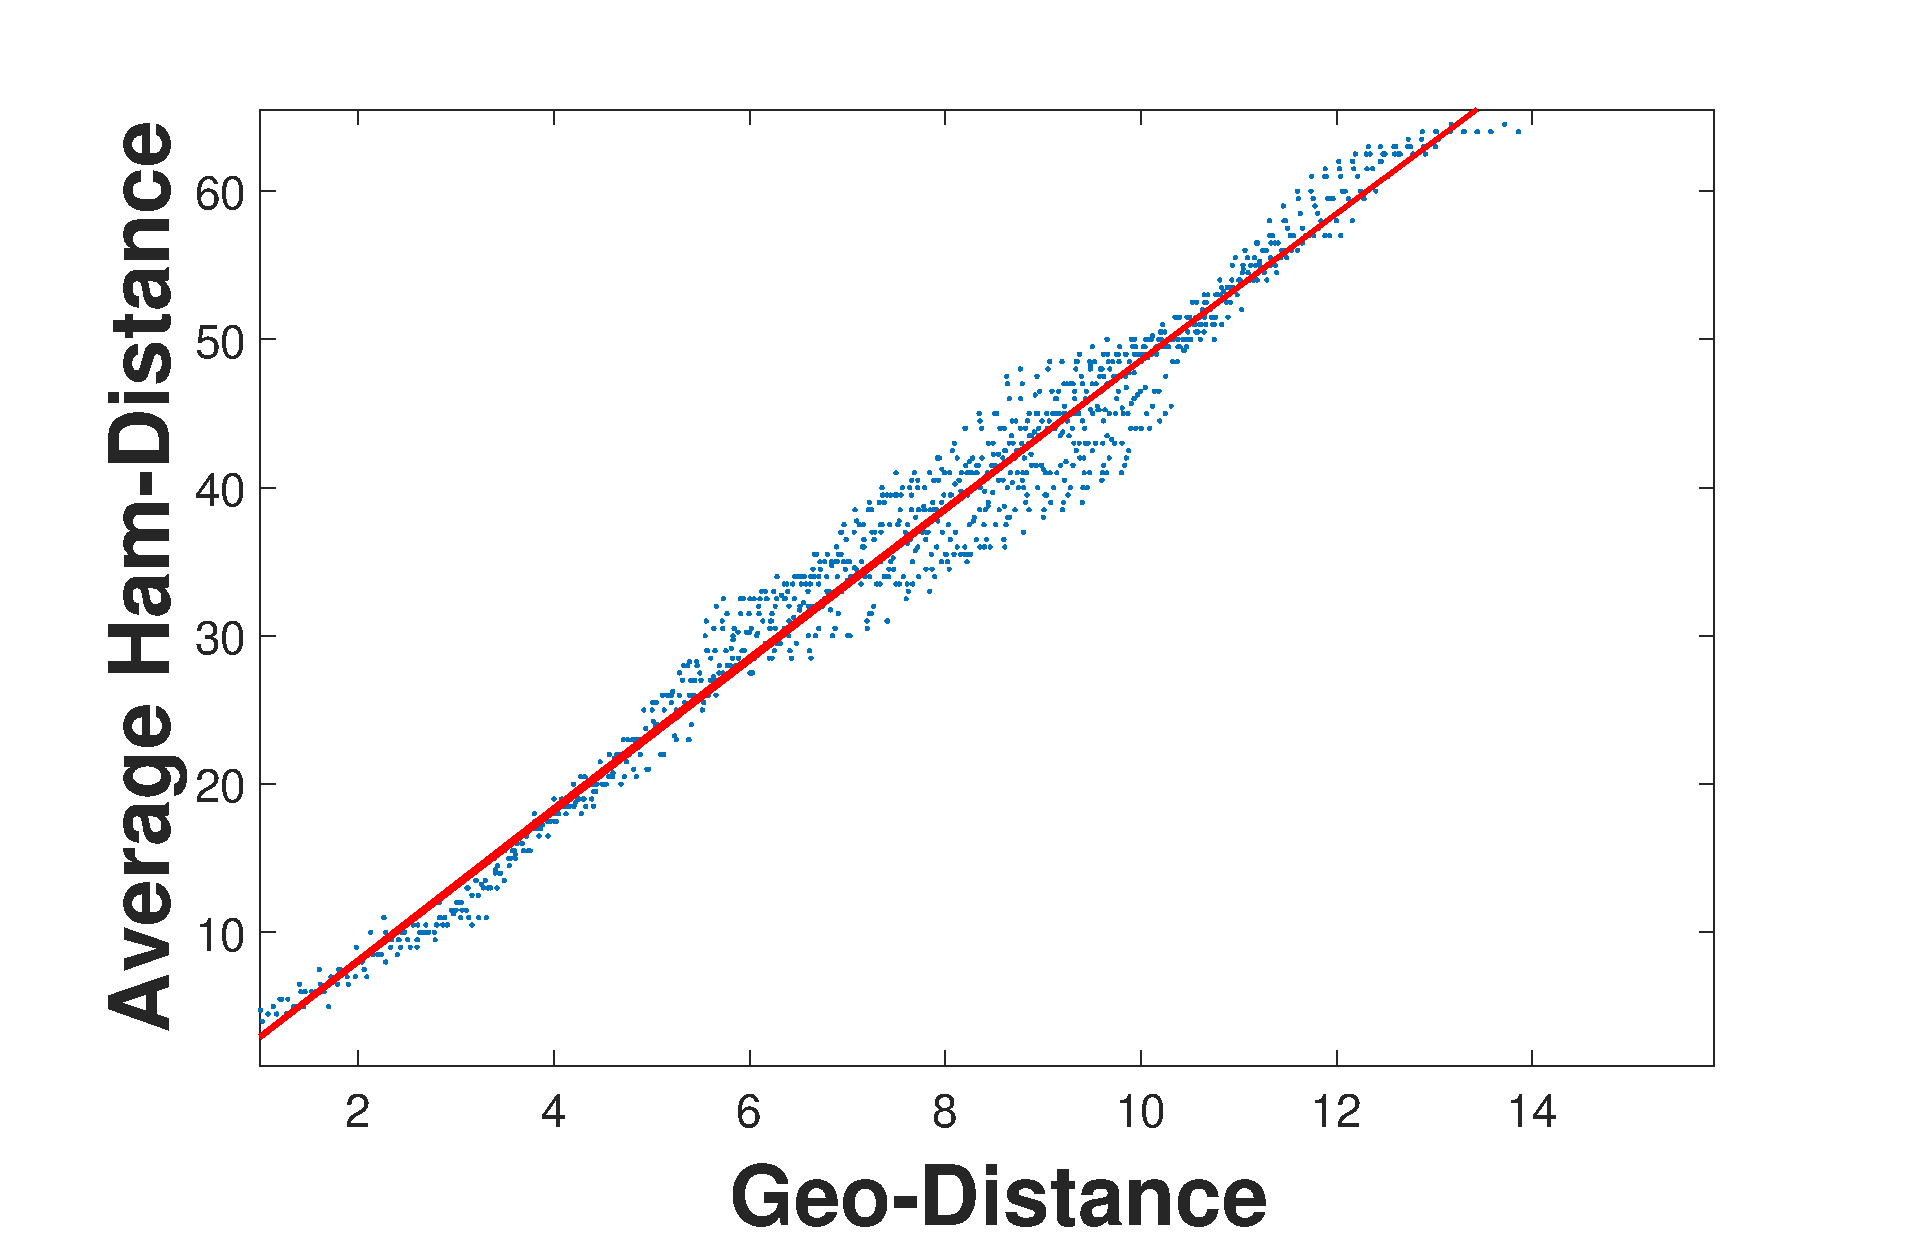
\includegraphics[height=2.85cm]{fig/Hamming2.eps}
		 \vspace{4mm}
	%	\caption{Average Hamming distance vs. Geographic distance.}
		\vspace{-4mm}
	\end{minipage}	
				\vspace{1mm}
			\caption{Relationship between Hamming distance and geographic distance.}
			\label{relationship}
		\vspace{-6mm}		
\end{figure}		
		
%  \ref{fig1} : ��figure��table���ƣ������У���д\caption{}��д\label{}��
From Fig. \ref{relationship} we can see that
the closer the two faces are in geographical distance, the smaller their Hamming distance is.
In other words, geographical distance is positively correlated with Hamming distance.  
For these two distances, we have the following observation:
 \begin{equation}
  \label{equation.1}
GD({f_i},{f_j}) \propto HD({f_i},{f_j})
 \end{equation}
 
Equation \eqref{equation.1} indicates that the Hamming distance between
two faces is approximately proportional with their geographical
distance. This is because longer geographical distance creates
more chances to cross bisectors, resulting in more flipped bit.  
So when the Hamming distance is close to zero, then the locations are very close to each other.  
Moreover, we do lots of simulation experiments to prove it. 
The result of the experiments can be seen in Fig.7 and Fig.8. It proves that Hamming distance is almost linear growth with geographical distance increasing. 
Given a query binary vector from multiple smartphones, we can estimate the location by retrieving the vectors in the beforehand database
and find the smallest Hamming distance. 
In other words, we can find the target location through by querying the smallest Hamming distance.



The basic ThunderLoc contains the three steps:

(1) Dividing the space into $p$ grid points : Suppose there is an acoustic source at the point $P{_i},i=1,...,p$, the $j-th$ smartphone $n{_j},j=1,...,N$ can compute the TDOA and get the sign of the TDOA.
Then we can get the binary code $C{_i,_j} \in \{ 0,1\}$ by the sign of TDOA. 
Combining the binary code of all $N$ smartphones, we can get a N-vector binary sequence $D{_i},i=1,...,p$. 
The database about $p$ discrete points is obtained, and an item in the database is ${S_i} = \{ D_i, P_i\} $.

(2) Computing the binary sequence $T$ of the target: When the acoustic source emits sound, 
all the smartphone nodes compute the TDOA, then get the sign of TDOA and determine the binary code. 
$ TDOA_{i}$  of the $ i-th $ smartphone can be computed by using time delay estimation algorithm(such as GCC), 
and the binary code of the ${i-th}$ smartphone can be defined by computing the sign of the TDOA:
 \begin{equation}\label{eq:eps}
Binary\_data_{i}=
\left\{\begin{matrix}
1 ,~~ $if$~~  TDOA_{i}\geq0;\\
0 ,~~ $if$~~  TDOA_{i}<0.
\end{matrix}\right.
 \end{equation}

(3) Processing the binary sequences $T$: Computing the Hamming distance between $T$ and each $D(i)$, the acoustic source position can  be found by searching the minimum of Hamming distance. However, it should be noted that in general there are several source points with the same
minimum value of Hamming distance. 
This is due to the finite estimate resolution which creates areas with the same Hamming distance. 
The final position estimate is the mean of all points with the minimum Hamming distance.  

We can calculate time complexity according to the three steps.
In step 1, we build the database, including calculating TDOA of a pair of microphones and getting its sign just use the linear time.
For each grid point we need to calculate TDOA of $N$ pairs of microphones and there exists $P$ grid points, so the time complexity in step 1  is $O \left( {PN} \right)$.
The time complexity of step 2 is $O \left( {N} \right)$ similarly.
In step 3, the time complexity of the search processing is  $O \left( {PN} \right)$. So the overall time complexity is $O \left( {PN} \right)$.

	
\begin{figure}[ht]
	\setlength{\abovecaptionskip}{0pt}
	\begin{minipage}[t]{0.45\linewidth}
		\centering
		\label{fig:subfig:a}		
		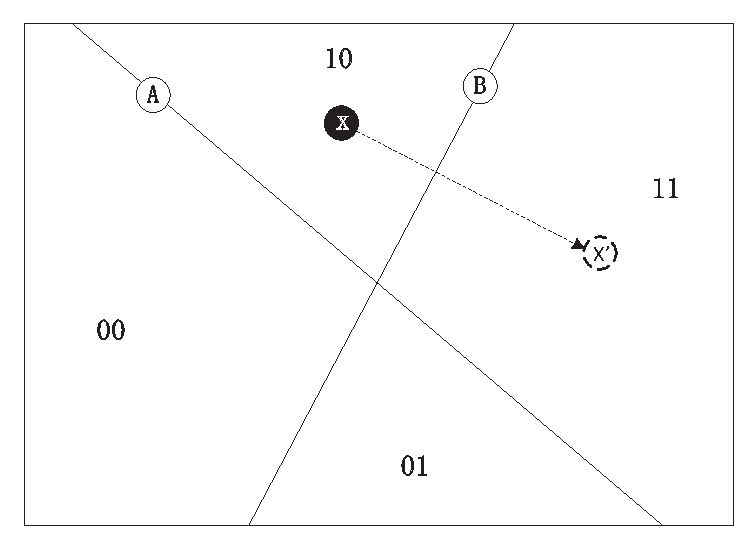
\includegraphics[height=2.8cm]{image/node.eps}
		\vspace{2mm}
		\subfigure{(a)}
		%\subfigure{(a) Measurement error.}
		\vspace{-2mm}
	\end{minipage}%
\hspace{0.5cm}
	\begin{minipage}[t]{0.45\linewidth}
		\centering
		\label{fig:subfig:b}
		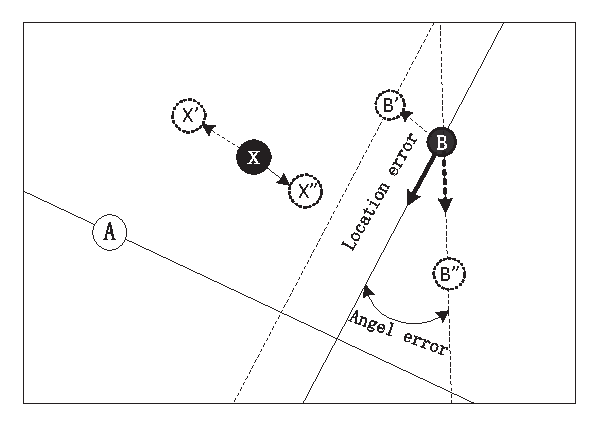
\includegraphics[height=2.8cm]{image/angleposition.eps}
		\vspace{2mm}
		\subfigure{(b)}
		%\subfigure{(b) Angle error and position error.}
		\vspace{-4mm}
	\end{minipage}	
	\vspace{1mm}
	\caption{The impact of variety of errors.}
	\label{Impact}
\end{figure}		
		
	\vspace{-4mm}
  
The bit flip problem for measurement data and the location and direction parameter errors have impact on the localization performance as shown in Fig. \ref{Impact}.
As shown in Fig. \ref{Impact}$(a)$, In case the measurement binary data from node B is flipped, the binary sequence $'10'$ is turned into $'11'$, reducing the accuracy of localization system. 
In Fig. \ref{Impact}$(b)$, if the position measurement or angle measurement of sensor B is inaccurate, 
there is a certain distance between actual position and estimated position.
According to the above, the basic Thunderloc is not suitable for the practical application. In the next section, 
we propose a robust localization solution against the measurement errors, position errors and orientation errors of smartphones.

  
\vspace{-4mm}
\subsection{Robust localization on server side}

In the practical application, the bit-flip problem mentioned before should be considered.
Moreover, the measurement error and  the uncertainty of node parameters have effects on the localization performance.
In this subsection, the robust version of ThunderLoc is devised to circumvent these problems.
The results we have obtained empirically indicate that the robust localization method can dramatically reduce the localization error under the practical application.

In order to improve the robustness of the localization system, the possible coordinates for the thunder are computed through selecting the K smallest Hamming distance instead of the minimum Hamming distance. 
Then, the centroid estimation method is utilized to set the center of gravity of  all the possible points as the estimated location of the thunder.

However, the selection of  the parameter $K$ is a difficult task. Deeply thinking the relation between the Hamming distance and the 2D geographic distance, the smaller Hamming distance is, the closer the coordinate region is to the target.
For each discrete point in localization space, the weight of each coordinate point is assigned based on Hamming distance.
Specially, the weight of each coordinate point is monotonic decreasing function of Hamming distance.

Gaussian function is adapted to weight discrete points according to the respective Hamming distance:
\begin{equation}
\label{weight}
{w_i} = exp(-HD(T,D_i)/N{\sigma ^2})
\end{equation}
where $\sigma$ is the parameter to decide the weighting strategy. 

Based on the normalized weight $\bar {w_i}$, the final estimated location of the thunder is estimated by computing the weight sum of all grid points:
\begin{equation}
 \label{normalized}
{\bar w_i} = \frac{{{w_i}}}{{\sum\limits_{i = 1}^P {{w_i}} }}
\end{equation}

\begin{equation}
 \label{estimated}
\hat x = \sum\limits_{i = 1}^P {{{\bar w}_i} \cdot {p_i}}
\end{equation}

Algorithm \textbf{1} illustrates the pseudo code of robust ThunderLoc method.
\begin{algorithm}
\caption{Robust ThunderLoc}
 \textbf{Input:} The location coordinates of all smartphones \\
\quad \quad \quad  The orientations of all the smartphones \\
\quad \quad \quad  Information about microphones $measure\_data$ \\
\textbf{Output:} Location of the thunder\\

\textbf{Step 1:} Database building:\\
\textbf{Step 2:} Computing the binary code $T$ of the thunder from the dual-channel acoustic signals: \\
\textbf{Step 3:} Processing the binary sequence: \\

(1) Computing Hamming distance for each point:\\
\For{$i \leftarrow 1$ \textbf{to} $p$}
 {
 ${HD(T,D(i))} = \sum\limits_{j = 1}^N {\left( {{T}(j) \oplus {D_i}(j)} \right)}$
 }
 
(2) Computing the weight of each grid point using Eq. \ref{weight} :\\
(3) Normalizing the weights and Estimating the source location using Eq. \ref{normalized} and  Eq. \ref{estimated}, respectively.\\
\end{algorithm}

%\vspace{-4mm}
Compared with the basic ThunderLoc, robust ThunderLoc leverages all possible points to locate the thunder.
Although the computing load increases, robust ThunderLoc has two benefits: (i) Avoiding the problem of selecting parameter $K$; (ii) More robust to measurement errors and node parameter errors.
Our evaluation in sections \ref{section:results} shows that robust localization method considerably enhances the robustness of localization system.

We can calculate time complexity of robust ThunderLoc according to the three steps. 
From the algorithm we can see  the time cost is the same as basic localization method in step 1 and step 2.
Besides, in step 3, we should calculate the normalized weighting of each point, and the corresponding time complexity is $O\left({P} \right)$.
At last step, we should calculate the location of the thunder by the weight sum of each grid point, and the corresponding time complexity is $O\left({P} \right)$.
The time complexity of robust ThunderLoc method is also $O\left( {PN} \right)$.
At the cost of $O\left({P} \right)$ time complexity more than basic ThunderLoc method, robust ThunderLoc method enhances system robustness.
The computing of Hamming distance is the core of the proposed ThunderLoc system, 
which can be effectively implemented via the Boolean XOR operation in the cloud computing platform with GPU and FPGA support.



